% Original schematic: faithful short paraphrases of inspected C12 and C10.
\documentclass[tikz,border=2pt]{standalone}
\usepackage{fontspec}
\setsansfont{Arial}
\usetikzlibrary{arrows.meta,shapes.misc}
\definecolor{blue}{HTML}{0072B2}
\definecolor{orange}{HTML}{B36B00}
\definecolor{ink}{HTML}{303843}
\begin{document}
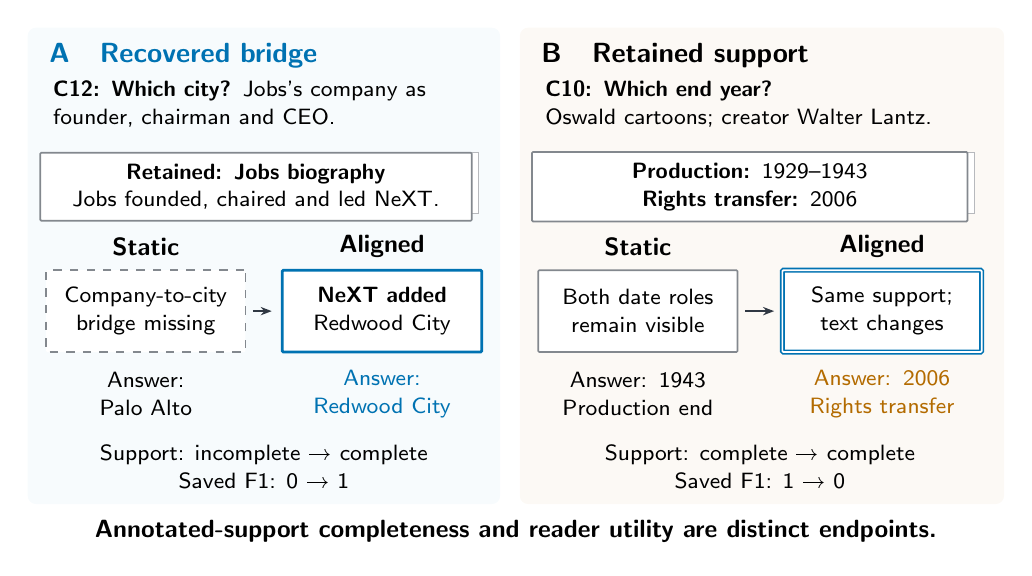
\begin{tikzpicture}[x=1cm,y=1cm,font=\sffamily\fontsize{8.5}{10}\selectfont,
 head/.style={font=\sffamily\bfseries\fontsize{10}{11}\selectfont,align=left,anchor=west},
 doc/.style={draw=ink!60,fill=white,line width=.6pt,rounded corners=.4pt,inner sep=4pt,align=center},
 flow/.style={-{Stealth[length=4pt]},draw=ink,line width=.7pt}]
\path[use as bounding box] (0,0) rectangle (12.4,6.6);
\fill[blue!3,rounded corners=3pt] (0,.55) rectangle (6.0,6.6);
\fill[orange!4,rounded corners=3pt] (6.25,.55) rectangle (12.4,6.6);
\node[head,text=blue] at (.15,6.25) {A\quad Recovered bridge};
\node[head] at (6.4,6.25) {B\quad Retained support};
\node[anchor=west,align=left,text width=5.65cm] at (.2,5.63)
 {\textbf{C12: Which city?} Jobs's company as\\founder, chairman and CEO.};
\node[anchor=west,align=left,text width=5.7cm] at (6.45,5.63)
 {\textbf{C10: Which end year?}\\Oswald cartoons; creator Walter Lantz.};
% Retained source cards; not verbatim quotations.
\draw[ink!35,fill=white] (.3,4.24) rectangle (5.72,5.02);
\node[doc,text width=5.2cm,minimum height=.78cm] at (2.9,4.58)
 {\textbf{Retained: Jobs biography}\\Jobs founded, chaired and led NeXT.};
\draw[ink!35,fill=white] (6.55,4.24) rectangle (12.03,5.02);
\node[doc,text width=5.25cm,minimum height=.78cm] at (9.17,4.58)
 {\textbf{Production:} 1929--1943\\\textbf{Rights transfer:} 2006};
\foreach \x/\t in {1.5/Static,4.5/Aligned,7.75/Static,10.85/Aligned}
 \node[font=\sffamily\bfseries\fontsize{9}{10}\selectfont] at (\x,3.82) {\t};
\node[doc,dashed,text width=2.25cm,minimum height=1.04cm] at (1.5,3.0)
 {Company-to-city\\bridge missing};
\node[doc,draw=blue,line width=1pt,text width=2.25cm,minimum height=1.04cm] at (4.5,3.0)
 {\textbf{NeXT added}\\Redwood City};
\draw[flow] (2.86,3.0)--(3.1,3.0);
\node[doc,text width=2.25cm,minimum height=1.04cm] at (7.75,3.0)
 {Both date roles\\remain visible};
\node[doc,draw=blue,double,text width=2.25cm,minimum height=1.04cm] at (10.85,3.0)
 {Same support;\\text changes};
\draw[flow] (9.11,3.0)--(9.48,3.0);
\node[align=center,text width=2.6cm] at (1.5,1.95) {Answer:\\Palo Alto};
\node[align=center,text width=2.6cm,text=blue] at (4.5,1.95) {Answer:\\Redwood City};
\node[align=center,text width=2.8cm] at (7.75,1.95) {Answer: 1943\\Production end};
\node[align=center,text width=2.8cm,text=orange] at (10.85,1.95) {Answer: 2006\\Rights transfer};
\node[align=center] at (3,1.02) {Support: incomplete → complete\\Saved F1: 0 → 1};
\node[align=center] at (9.3,1.02) {Support: complete → complete\\Saved F1: 1 → 0};
\node[font=\sffamily\bfseries\fontsize{9}{10}\selectfont] at (6.2,.2)
 {Annotated-support completeness and reader utility are distinct endpoints.};
\end{tikzpicture}
\end{document}
